\chapter{傅里叶变换}

本章起至第六章介绍傅里叶变换。
傅里叶变换是对信号的处理,不描述系统,但它是后续讨论系统传递函数和其他各种变换的基础。

本章从三角级数和傅里叶级数入手,引出傅里叶变换。
信号与系统中的傅里叶变换着重性质和应用,不太重视来源和推导过程,这部分是在微积分中讲授,所以学习本章最好配合微积分教材中的级数章节,特别是三角级数、傅里叶级数和傅里叶积分,相互印证着看。
本章最后给出Python应用,介绍如何使用Python求解傅里叶变换和逆变换。

本章要点:
\begin{itemize}
    \item 傅里叶变换。
\end{itemize}

~

本章至第六章的结构:
\begin{itemize}
    \item {\bf 第四章 \, 傅里叶变换}:介绍连续时域的傅里叶变换(CTFT),系统地讲述傅里叶变换的概念和性质,是后续两章的基础;
    \item {\bf 第五章 \, 系统的频率分析}:从频率角度考察系统,算作是CTFT的一个简单应用;
    \item {\bf 第六章 \, 离散傅里叶变换}:介绍离散傅里叶变换(DFT),由于现代数字处理芯片的使用,所以DFT是学习整个傅里叶变换的目标。
\end{itemize}

\newpage
\section{周期信号的傅里叶级数型}

本节简单介绍周期信号的傅里叶级数,具体推导参见《微积分笔记》。

本节要点:
\begin{itemize}
    \item 掌握傅里叶级数的三角级数形式;
    \item 掌握傅里叶级数的复指数形式;
    \item 理解傅里叶级数的量纲;
    \item 熟练掌握周期信号的复指数展开。
\end{itemize}

%============================================================
\subsection{三角级数展开}

{\bf 三角级数展开}:当周期为$T$的信号$x\left( t \right) $满足狄利克雷收敛条件时,其在周期内可以展开成三角级数,即无穷项余弦函数的叠加,且收敛于该周期信号:
\[
x\left( t \right) =A_0+\sum_{n=1}^{+\infty}{A_n\cos \left( \omega _nt+\varphi _n \right)}
\]
\begin{itemize}
    \item $A_0,A_n$:{\bf 傅里叶系数},$A_0$表示信号的{\bf 直流分量}或{\bf 基频分量};
    \item $\omega _n=n\omega _0$:对应余弦项的{\bf 角频},称$\omega _0=2\pi /T$为{\bf 基频};
    \item $\varphi _n$:对应余弦项的{\bf 初始相位},简称{\bf 相位}。
\end{itemize}

数学上,周期函数都能展开成三角级数,但不一定收敛,即便收敛也不一定收敛至原函数。
如果周期函数满足狄利克雷充分条件,即周期函数必须在一个包含原点的最小周期内连续,或只有有限个一类间断点,而且只有有限个极值点,则三角级数收敛在原函数。
这样的三角级数称为傅里叶级数。

周期信号展开成三角级数后,对信号又多了一种描述方法,即以频率$\omega _n$为自变量,幅值和初相为因变量的两个函数$A\left( \omega _n \right) ,\varphi \left( \omega _n \right) $:
\[
x=x\left( t \right) ,T=\frac{2\pi}{\omega _0} \quad \Leftrightarrow \quad \begin{cases}
	A=A\left( \omega _n \right)\\
	\varphi =\varphi \left( \omega _n \right)\\
\end{cases}
\]
在图形方面,原本只有时域上的波形图,现在多了两张频域上的图形,称为{\bf 幅频图}(amplitude spectrum) 和{\bf 相频图}(phase spectrum) ,统称为{\bf 频谱图}。

%============================================================
\subsection{复指数级数展开}

{\bf 复指数级数展开}:当周期为$T$的信号$x\left( t \right) $满足狄利克雷收敛条件时,其在周期内可以展开成复指数级数形式,且收敛于该周期信号:
\begin{align*}
&x\left( t \right) =C_0+\sum_{n=-\infty ,n\ne 0}^{+\infty}{\left( C_ne^{i\omega _nt} \right)} \\
&\begin{cases}
	C_0=\frac{1}{T}\int_{-\frac{T}{2}}^{\frac{T}{2}}{x\left( t \right) dt}\\
	C_n=\frac{1}{T}\int_{-\frac{T}{2}}^{\frac{T}{2}}{x\left( t \right) e^{-i\omega _nt}dt}\\
\end{cases}
\end{align*}
\begin{itemize}
    \item $C_0,C_n$:{\bf 傅里叶系数的复数形式};
    \item $\omega _n=n\omega _0$:对应{\bf 复指数项的角频},$\omega _0=2\pi /T$称为{\bf 基频}。
\end{itemize}
该级数称为{\bf 傅里叶级数的复数形式}。
此时的信号可以用以频率$\omega _n$为自变量的复函数$C=C\left( \omega _n \right) $表示:
\[
x=x\left( t \right) ,T=\frac{2\pi}{\omega _0} \quad \Leftrightarrow \quad C=C\left( \omega _n \right)
\]

由欧拉公式可得三角级数和复指数级数的关系:
\begin{align*}
&x\left( t \right) =A_0+\sum_{n=1}^{+\infty}{A_n\cos \left( \omega _nt+\varphi _n \right)}=C_0+\sum_{n=-\infty ,n\ne 0}^{+\infty}{\left( C_ne^{i\omega _nt} \right)} \\
&\begin{cases}
	A_0=C_0\\
	A_n=2\left| C_n \right|\\
	\varphi _n=\angle C_n\\
\end{cases}
\end{align*}
且常称$A_n\cos \left( \omega _nt+\varphi _n \right) $为{\bf {\it n}次谐波}({\it n}th harmonic)。

由于信号是周期性,所以频率虽然是无穷多,但还是取离散的值$n\omega _0$。复指数形式中,首先将相位和振幅合并成一个复数;其次,通过引入“负频率”制造一对共轭对,一起表示该频率的{\it n}次谐波分量$C_ne^{i\omega _nt}+C_{-n}e^{i\omega _{-n}t}=A_n\cos \left( n\omega _0t+\varphi _n \right) $。
最后需要注意的是,不同的周期信号,在时域上表现为不同的波形$x\left( t \right) $,在频域上则表现为不同的傅里叶系数$C_n$,所以频域的频谱图是和时域的波形图一样真实的存在。

\begin{theorem}[Parseval定理]
周期信号的功率为$P=\frac{1}{T}\int_{-\frac{T}{2}}^{\frac{T}{2}}{\left| x\left( t \right) \right|^2dt}$,若信号展开成傅里叶级数,功率可以表示为:
\[
P=\sum_{n=-\infty}^{+\infty}{\left| C_n \right|^2}
\]
\end{theorem}

%============================================================
\subsection{傅里叶级数的量纲}

物理上,只有具有相同量纲的变量才可以作加减,所以$x\left( t \right) ,A_0,A_n$具有相同的量纲,$\omega _n$的量纲是$\mathrm{rad}\cdot \mathrm{s}^{-1}$,$\varphi _n$的量纲是$\mathrm{rad}$。对于复指数级数,通过引入负频率,我们用一对共轭复数$C_ne^{i\omega _nt},C_{-n}e^{i\omega _{-n}t}$对表示信号在某个频率的成分,即:
\[
C_ne^{i\omega _nt}+C_{-n}e^{i\omega _{-n}t}=2\left| C_n \right|\cos \left( \omega _nt+\angle C_n \right) =A_n\cos \left( \omega _nt+\varphi _n \right)
\]
所以,$x\left( t \right) ,C_n$具有相同量纲。

虽然$x\left( t \right) ,C_n$具有相同量纲,但因为它们总是以共轭对的形式出现,所以单独$C_n$讨论没有意义,只需要考察正频率部分即可。

\begin{tcolorbox}
量纲的概念需要贯穿始终。
\end{tcolorbox}

%============================================================
\subsection{复指数级数展开的步骤}

周期信号展开成傅里叶级数(这里指复指数形式)时,只要级数项的个数足够多就能足够描述原信号。

展开步骤为:
\begin{enumerate}
    \item 根据信号周期$T$确定基频及各个谐波频率:
    \[
    \omega _0=\frac{2\pi}{T} \qquad \omega _n=n\omega _0=\frac{2n\pi}{T}
    \]
    \item 计算直流分量和谐波的傅里叶系数:
    \[
    C_0=\frac{1}{T}\int_{-\frac{T}{2}}^{\frac{T}{2}}{x\left( t \right) dt} \qquad C_n=\frac{1}{T}\int_{-\frac{T}{2}}^{\frac{T}{2}}{x\left( t \right) e^{-i\omega _nt}dt}
    \]
    \item 计算得到信号的展开式:
    \[
    x\left( t \right) =C_0+\sum_{n=\pm 1}^{\pm \infty}{\left( C_ne^{i\omega _nt} \right)}
    \]
\end{enumerate}

通过对量纲的分析可知,即便采用复指数形式展开,依然必定是不含虚数的!
也就是说,$C_n$可以有虚部,但$x\left( t \right) $的展开结果必然是通过$\pm n$抵消虚部。

%============================================================
\subsection{例}

~

\begin{example}
假设如下图方波,求其傅里叶级数,并用Python画图验证。
\begin{figure}[ht]
\centering
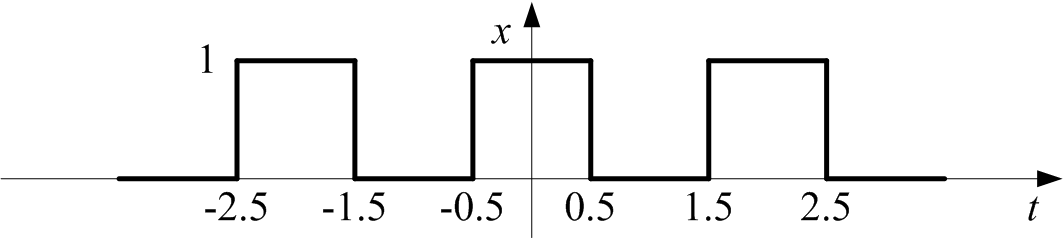
\includegraphics[height=2cm]{4.1.5-1.png}
\end{figure}
\end{example}

易得$T=2,\omega _0=\pi ,\omega _n=n\pi $,计算傅里叶系数:
\begin{align*}
C_0&=\frac{1}{T}\int_{-\frac{T}{2}}^{\frac{T}{2}}{x\left( t \right) dt}=\frac{1}{2}\int_{-1}^1{x\left( t \right) dt}=\frac{1}{2}\int_{-0.5}^{0.5}{dt}=\frac{1}{2} \\
C_n&=\frac{1}{T}\int_{-\frac{T}{2}}^{\frac{T}{2}}{x\left( t \right) e^{-i\omega _nt}dt}=\frac{1}{2}\int_{-0.5}^{0.5}{e^{-in\pi t}dt} =\frac{i}{2n\pi}\left( e^{-\frac{in\pi}{2}}-e^{\frac{in\pi}{2}} \right) \\
&=\frac{i}{2n\pi}\left[ \cos \left( -\frac{n\pi}{2} \right) +i\sin \left( -\frac{n\pi}{2} \right) -\cos \left( \frac{n\pi}{2} \right) -i\sin \left( \frac{n\pi}{2} \right) \right] \\
&=\frac{1}{n\pi}\sin \left( \frac{n\pi}{2} \right)
\end{align*}
由于$\sin \left( \frac{n\pi}{2} \right) =0,n=0,\pm 2,\pm 4,\cdots $,所以跳过偶数以减小计算量,得到最终的傅里叶级数:
\[
x\left( t \right) =C_0+\sum_{n=\pm 1,odd}^{\pm \infty}{\left[ C_n\cdot e^{in\pi t} \right]}=\frac{1}{2}+\sum_{n=1,odd}^{+\infty}{\left[ 2\cdot \frac{\sin \left( n\pi /2 \right)}{n\pi}\cdot \cos \left( n\pi t \right) \right]}
\]
用Python分别对累加至3、8、20、100次谐波的傅里叶级数作图如下,谐波叠加越多,越能近似原信号。
\begin{figure}[h]
\centering
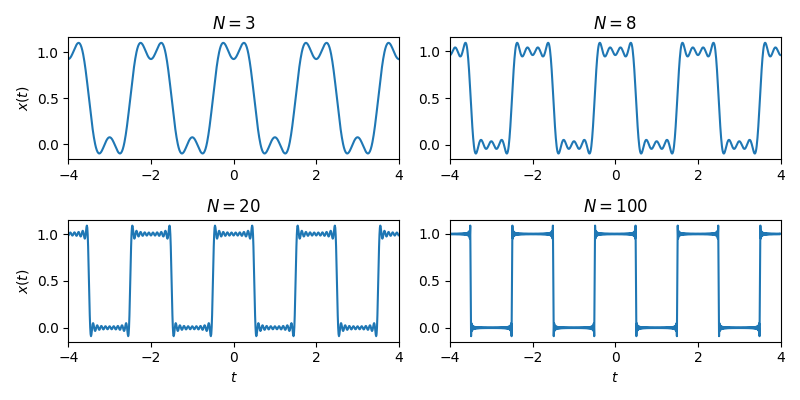
\includegraphics[height=5cm]{4.1.5-2.png}
\end{figure}

\begin{python}
t  = np.arange(-4, 4, 0.01)
x1 = np.full_like(t, 0.5, dtype=np.float32)
N = 3
for n in range(1,N+1,2):
    x1 += 2/n/np.pi * np.sin(n*np.pi/2) * np.cos(n*np.pi*t)
    pass

axs[0][0].plot(t, x1)
\end{python}

\begin{tcolorbox}
由于时域方波有不连续点,不满足狄利克雷收敛条件,所以在这些间断点,傅里叶级数和原函数有9\%的误差,称为{\bf Gibbs现象}。
\end{tcolorbox}

~

\begin{example}
假设如下图信号,求傅里叶级数,当$T=2,a=0.5$时,用Python作图验证。
\begin{figure}[h]
\centering
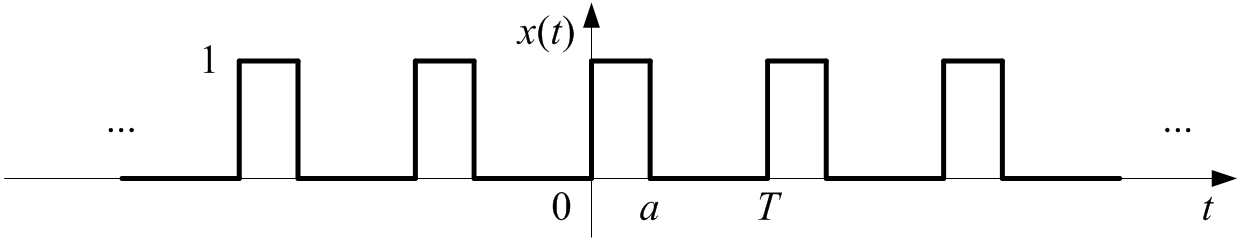
\includegraphics[height=2cm]{4.1.5-3.png}
\end{figure}
\end{example}

计算傅里叶系数:
\begin{align*}
&C_0=\frac{1}{T}\int_{-\frac{T}{2}}^{\frac{T}{2}}{x\left( t \right) dt}=\frac{1}{T}\int_0^a{dt}=\frac{a}{T} \\
&C_n=\frac{1}{T}\int_{-\frac{T}{2}}^{\frac{T}{2}}{x\left( t \right) e^{-i\omega _nt}dt}=\frac{1}{T}\int_0^a{e^{-in\frac{2\pi}{T}t}dt} =\frac{i}{2n\pi}\left( e^{-\frac{i2an\pi}{T}}-1 \right)
\end{align*}
得傅里叶级数:
\[
x\left( t \right) =C_0+\sum_{n=\pm 1}^{\pm \infty}{\left[ C_n\cdot e^{in\frac{2\pi}{T}t} \right]}=\frac{a}{T}+\sum_{n=1}^{+\infty}{\frac{\sin \frac{2n\pi t}{T}-\sin \frac{2n\pi \left( t-a \right)}{T}}{n\pi}}
\]
\begin{figure}[h]
\centering
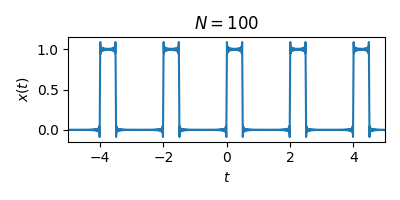
\includegraphics[height=3cm]{4.1.5-4.png}
\end{figure}

~

\begin{example}
设如下图信号,求傅里叶级数,用Python作图验证。
\begin{figure}[h]
\centering
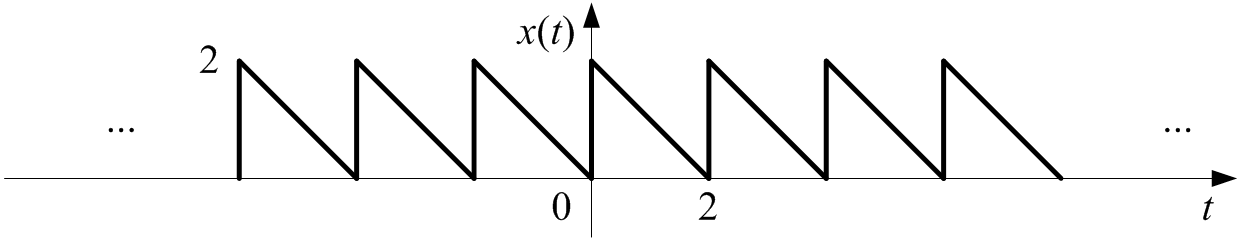
\includegraphics[height=2cm]{4.1.5-5.png}
\end{figure}
\end{example}

显然,信号有$x\left( t \right) =2-t,T=2$,计算傅里叶系数:
\begin{align*}
&C_0=\frac{1}{T}\int_{-\frac{T}{2}}^{\frac{T}{2}}{x\left( t \right) dt}=\frac{1}{2}\int_0^2{\left( 2-t \right) dt}=1 \\
&C_n=\frac{1}{T}\int_{-\frac{T}{2}}^{\frac{T}{2}}{x\left( t \right) e^{-i\omega _nt}dt}=\frac{1}{2}\int_0^2{\left( 2-t \right) e^{-i\omega _nt}dt}=\frac{1-i2\omega _n-e^{-i2\omega _n}}{2{\omega _n}^2}
\end{align*}
得傅里叶级数:
\begin{align*}
x\left( t \right) &=C_0+\sum_{n=\pm 1}^{\pm \infty}{\left[ C_n\cdot e^{in\omega _nt} \right]} \\
&=1+\sum_{n=1}^{+\infty}{\frac{\cos \left( n\pi t \right) +2n\pi \sin \left( n\pi t \right) -\cos \left( n\pi \left( t-2 \right) \right)}{\left( n\pi \right) ^2}}
\end{align*}
\begin{figure}[h]
\centering
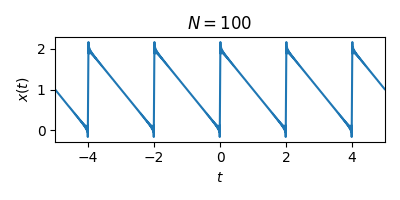
\includegraphics[height=3cm]{4.1.5-6.png}
\end{figure}






\newpage
\section{非周期信号的傅里叶变换}

本节介绍非周期信号的傅里叶变换。
傅里叶变换是频域分析的重要方法,也是各种其他变换的基础。

本节要点:
\begin{itemize}
    \item 深入理解傅里叶变换及其物理意义;
    \item 理解傅里叶变换的量纲;
    \item 理解傅里叶变换的条件;
    \item 熟悉傅里叶变换的极坐标形式;
    \item 了解傅里叶级数和傅里叶变换的关系。
\end{itemize}

\begin{tcolorbox}
建议和《微积分》课程中的傅里叶积分对比着学习!
\end{tcolorbox}

%============================================================
\subsection{傅里叶变换的概念}

\begin{definition}[傅里叶变换]
若非周期信号$x\left( t \right) $满足:
\begin{itemize}
    \item 任一有限区域上满足狄利克雷收敛条件,
    \item 整个实数域绝对可积,即$\int_{-\infty}^{+\infty}{\left| x\left( t \right) \right|dt}$收敛,
\end{itemize}
则有:
\[
x\left( t \right) =\frac{1}{2\pi}\int_{-\infty}^{+\infty}{\left[ \int_{-\infty}^{+\infty}{x\left( t \right) e^{-i\omega t}dt} \right] e^{i\omega t}d\omega}
\]
对$x\left( t \right) $所有的连续点成立,称为{\bf $x\left( t \right) $的傅里叶积分},在间断点$t_0$处,可以用$\frac{1}{2}\left[ x\left( {t_0}^+ \right) +x\left( {t_0}^- \right) \right] $代替。
同时称$\int_{-\infty}^{+\infty}{x\left( t \right) e^{-i\omega t}dt}$为{\bf 信号$x\left( t \right) $的傅里叶变换}(Fourier transform,FT),记为$X\left( \omega \right) $即:
\[
X\left( \omega \right) =\int_{-\infty}^{+\infty}{x\left( t \right) e^{-i\omega t}dt}
\]
相应地称
\[
x\left( t \right) =\frac{1}{2\pi}\int_{-\infty}^{+\infty}{X\left( \omega \right) e^{i\omega t}d\omega}
\]
为{\bf 傅里叶逆变换}。
信号及其傅里叶变换形式通常记为:
\[
x\left( t \right) \overset{\mathscr{F}}{\leftrightarrow}X\left( \omega \right)
\]
\end{definition}

傅里叶变换是针对非周期信号而言的,所以没有基频这个概念,频率是一片连续的范围,与之相对的是周期信号的傅里叶级数的频率是无穷个离散值,可以想象成“连续谱”vs“线状谱”,傅里叶级数中的系数也从离散的$C_n$变成连续的$X\left( \omega \right) $。

如果信号在时域占满整个实数域$\mathbb{R} $,则对应傅里叶变换的频率在一个区间$\left( -\omega _0,+\omega _0 \right) $,相反,如果信号在时域是一个区间$\left( t_1,t_2 \right) $,则在频域将占满整个频率$\mathbb{R} $,即信号要么时域有限,要么频域有限,通常来讲,一般物理信号都是时域有限信号,所以是频域无限。

傅里叶变换和逆变换的对称性可知,只要信号能有傅里叶变换,则必有其傅里叶变换绝对可积,即$\int_{-\infty}^{+\infty}{\left| X\left( \omega \right) \right|d\omega}$收敛。

%============================================================
\subsection{傅里叶变换的量纲}

从定义式易得$X\left( \omega \right) $的量纲是信号的量纲乘以时间的量纲,或者说是信号的量纲除以频率的量纲$\mathrm{D}_x\cdot \mathrm{Hz}^{-1}$,这点是和傅里叶级数的区别。
{\bf $X\left( \omega \right) $的物理意义可以理解为单位频率的信号,或者说信号的频率密度。}
有些教材中会使用“信号分布在低频”这样的说法!

%============================================================
\subsection{傅里叶级数和傅里叶变换对比}

傅里叶级数和傅里叶变换的对比见下表:

\begin{table}[h]
\centering
% \caption{表头}
\begin{tabular}{ccc}
    \toprule
    & 傅里叶级数 & 傅里叶变换\\
    \midrule
    目标函数 & 周期函数 & 非周期函数\\
    展开 & $x\left( t \right) =\sum_{n=-\infty}^{+\infty}{\left( C_ne^{i\omega _nt} \right)}$ & $x\left( t \right) =\frac{1}{2\pi}\int_{-\infty}^{+\infty}{X\left( \omega \right) e^{i\omega t}d\omega}$\\
    角频 & 离散值,$\omega _n=n\omega _0=n\frac{2\pi}{T}$ & 连续值,$\omega \in \mathbb{R} $\\
    系数 & $C_n=\frac{1}{T}\int_{-\frac{T}{2}}^{\frac{T}{2}}{x\left( t \right) e^{-i\omega _nt}dt}$ & $X\left( \omega \right) =\int_{-\infty}^{+\infty}{x\left( t \right) e^{-i\omega t}dt}$\\
    \bottomrule
\end{tabular}
\end{table}

总之,对于周期信号的傅里叶级数,角频和系数的取值都是离散值,对于非周期信号的傅里叶变换,角频和系数的取值都是连续值。
这点可以类比为离散信号和连续信号。

%============================================================
\subsection{傅里叶变换的极坐标形式}

由于傅里叶变换有复指数项,所以结果一般是一个复数函数,可以变成极坐标形式:
\begin{align*}
X\left( \omega \right) &=\int_{-\infty}^{+\infty}{x\left( t \right) e^{-i\omega t}dt} \\
&=\int_{-\infty}^{+\infty}{x\left( t \right) \cos \left( \omega t \right) dt}+i\int_{-\infty}^{+\infty}{-x\left( t \right) \sin \left( \omega t \right) dt} \\
&=R\left( \omega \right) +iI\left( \omega \right)
\end{align*}
于是:
\begin{align*}
&\therefore \begin{cases}
	X\left( \omega \right) =\sqrt{R^2\left( \omega \right) +I^2\left( \omega \right)}\\
	\angle X\left( \omega \right) =\mathrm{arc}\tan \frac{I\left( \omega \right)}{R\left( \omega \right)}\\
\end{cases} \\
&\therefore X\left( \omega \right) =\left| X\left( \omega \right) \right|\cdot e^{i\angle X\left( \omega \right)}
\end{align*}
可以做类比:
\begin{itemize}
    \item $X\left( \omega \right) $:相当于傅里叶级数中的复指系数$C_n$;
    \item $\left| X\left( \omega \right) \right|$:相当于傅里叶级数中的幅度$A_n$;
    \item $\angle X\left( \omega \right) $:相当于傅里叶级数中的相位$\varphi _n$。
\end{itemize}

%============================================================
\subsection{广义傅里叶变换}

对于有些函数,如$x\left( t \right) =1,x\left( t \right) =\sin t$等,由于不满足狄利克雷条件,没有严格意义上的傅里叶变换,但可以通过单位冲激结合傅里叶变换的性质定义广义傅里叶变换。

单位冲激的傅里叶变换:
\begin{align*}
&\because \int_{-\infty}^{+\infty}{\delta \left( t \right) e^{i\omega t}dt}=\int_{-\infty}^{+\infty}{\delta \left( t \right) dt}=1 \\
&\therefore \delta \left( t \right) \leftrightarrow 1
\end{align*}
通过Duality,$x\left( t \right) =1$的广义傅里叶变换:
\[
1\leftrightarrow 2\pi \delta \left( \omega \right)
\]
以上只是一个例子,通过$\delta \left( t \right) $的傅里叶变换和傅里叶变换的性质,我们可以求得很多函数的广义傅里叶变换。

%============================================================
\subsection{傅里叶变换的性质}

{\bf 奇偶性}

如果$x\left( t \right) $是偶函数,则其傅里叶变换是实函数,如果$x\left( t \right) $是奇函数,则其傅里叶变换是纯虚函数,除此之外,一般傅里叶变换是复变函数。
\begin{align*}
&x\left( t \right) \text{ is even} \quad \Rightarrow \quad X\left( \omega \right) =\int_{-\infty}^{+\infty}{x\left( t \right) \cos \left( \omega t \right) dt} \\
&x\left( t \right) \text{ is odd} \quad \Rightarrow \quad X\left( \omega \right) =-i\int_{-\infty}^{+\infty}{x\left( t \right) \sin \left( \omega t \right) dt}
\end{align*}

{\bf 线性性}(由于积分的线性性,不证自明)
\[
ax\left( t \right) +by\left( t \right) \leftrightarrow aX\left( \omega \right) +bY\left( \omega \right)
\]

{\bf 时移性、频移性}(积分变量做一个变换即可证明)
\begin{align*}
&x\left( t-t_1 \right) \leftrightarrow X\left( \omega \right) e^{i\omega t_1} \\
&e^{i\omega t_1}x\left( t \right) \leftrightarrow X\left( \omega -\omega _1 \right)
\end{align*}

“时移性”表示信号在时域的延迟对傅里叶变换的结果是所有频率分量都慢了一个相位(即旋转),大小不变。
物理上讲,因为时间起点是人为设定的,所以信号的时移应具有FT的某种不变性。

{\bf 时展性}(积分变量做一个变换即可证明)
\begin{align*}
&x\left( at \right) \leftrightarrow \frac{1}{a}X\left( \frac{\omega}{a} \right) \\
&x\left( -t \right) \leftrightarrow -X\left( -\omega \right) =\bar{X}\left( \omega \right)
\end{align*}

“时展性”表示对时域的尺度变换对导致频域的尺度“相反地”变换。
这个容易理解,时域尺缩表示信号变化加快,自然频率尺扩,即高频分量增加。

{\bf 三角律}(频移性结合欧拉公式即可证明)
\begin{align*}
&x\left( t \right) \cos \omega _1t\leftrightarrow \frac{1}{2}\left[ X\left( \omega +\omega _1 \right) +X\left( \omega -\omega _1 \right) \right] \\
&x\left( t \right) \sin \omega _1t\leftrightarrow \frac{i}{2}\left[ X\left( \omega +\omega _1 \right) -X\left( \omega -\omega _1 \right) \right]
\end{align*}

{\bf 时域的微分和积分、频域的微分}
\begin{align*}
&\frac{d^nx\left( t \right)}{dt^n}\leftrightarrow \left( i\omega \right) ^n\cdot X\left( \omega \right) \\
&\int_{-\infty}^t{x\left( \tau \right) d\tau}\leftrightarrow \frac{1}{i\omega}\cdot X\left( \omega \right) \\
&\left( \frac{t}{i} \right) ^n\cdot x\left( t \right) \leftrightarrow \frac{d^nX\left( \omega \right)}{d\omega ^n}
\end{align*}

时域微分公式的前提是$\underset{t\rightarrow \pm \infty}{\lim} x\left( t \right) =0$。
时域积分通常来讲只有广义傅里叶变换,$\int_{-\infty}^t{x\left( \tau \right) d\tau}\leftrightarrow \frac{1}{i\omega}\cdot X\left( \omega \right) +\pi X\left( 0 \right) \delta \left( \omega \right) $。
特别地当时域信号没有直流分量时($X\left( 0 \right) =0$),才能得到上述公式。

{\bf 卷积性}
\begin{align*}
&x\left( t \right) \ast y\left( t \right) \leftrightarrow X\left( \omega \right) \cdot Y\left( \omega \right) \\
&x\left( t \right) \cdot y\left( t \right) \leftrightarrow \frac{1}{2\pi}\left[ X\left( \omega \right) \ast Y\left( \omega \right) \right]
\end{align*}

{\bf Parseval定理}
\begin{align*}
&\int_{-\infty}^{+\infty}{x\left( t \right) y\left( t \right) dt}=\frac{1}{2\pi}\int_{-\infty}^{+\infty}{\bar{X}\left( \omega \right) Y\left( \omega \right) d\omega} \\
&\int_{-\infty}^{+\infty}{x^2\left( t \right) dt}=\frac{1}{2\pi}\int_{-\infty}^{+\infty}{\left| X\left( \omega \right) \right|^2d\omega}
\end{align*}

{\bf Duality}
\[
X\left( t \right) \leftrightarrow 2\pi x\left( -\omega \right)
\]

%============================================================
\subsection{例}

\begin{example}
若有指数信号$x\left( t \right) =e^{-bt}u\left( t \right) $,求其傅里叶变换。
\end{example}

\begin{align*}
X\left( \omega \right) &=\int_{-\infty}^{+\infty}{x\left( t \right) e^{-i\omega t}dt}=\int_{-\infty}^{+\infty}{e^{-\left( b+i\omega \right) t}dt} \\
&=-\frac{1}{b+i\omega}\left[ \left. e^{-\left( b+i\omega \right) t} \right|_{0}^{+\infty} \right]
\end{align*}
当$b>0$时,有$\underset{t\rightarrow +\infty}{\lim} e^{-bt}=0$,则:
\[
X\left( \omega \right) =\frac{1}{b+i\omega}
\]
傅里叶变换是一个复数。
当$b\leqslant 0$时,$e^{-bt}$不收敛,信号不满足绝对可积条件,无傅里叶变换。

~

\begin{example}
若如下单方波信号,求其傅里叶变换,并分析脉宽和傅里叶变换之间的关系。
\[
p_{\tau}\left( t \right) =\begin{cases}
	1,t\in \left[ -\frac{\tau}{2},\frac{\tau}{2} \right]\\
	0,t\notin \left[ -\frac{\tau}{2},\frac{\tau}{2} \right]\\
\end{cases}
\]
\end{example}

先求傅里叶变换:
\begin{align*}
X\left( \omega \right) &=\int_{-\infty}^{+\infty}{x\left( t \right) e^{-i\omega t}dt}=\int_{-\frac{\tau}{2}}^{\frac{\tau}{2}}{e^{-i\omega t}dt} \\
&=\frac{1}{-i\omega}\left. e^{-i\omega t} \right|_{-\frac{\tau}{2}}^{\frac{\tau}{2}}=\frac{1}{-i\omega}\left( e^{-i\omega \frac{\tau}{2}}-e^{i\omega \frac{\tau}{2}} \right) \\
&=\frac{2}{\omega}\sin \frac{\omega \tau}{2}=\tau \frac{\sin \frac{\omega \tau}{2}}{\frac{\omega \tau}{2}}=\tau \mathrm{sinc}\frac{\omega \tau}{2\pi}
\end{align*}
由于信号是一个偶信号,傅里叶变换的结果是一个实数,它的相位永远只有0°和180°两个值。

以$\tau =0.5,\tau =1.5$两个脉宽的单方波信号为例,幅频图和相频图如下。

\begin{python}
w   = np.arange(-10*np.pi, 10*np.pi, 0.01)
tau = 0.5; X1 = tau * np.sinc(w*tau / 2 / np.pi)
tau = 1.5; X2 = tau * np.sinc(w*tau / 2 / np.pi)

plot_mag_phs(w, np.abs(X1), np.angle(X1, deg=True),
             axs[0][0], axs[1][0], title=r'$\tau =0.5$', ...)
plot_mag_phs(w, np.abs(X2), np.angle(X2, deg=True),
             axs[0][1], axs[1][1], title=r'$\tau =1.5$', ...)
\end{python}

\begin{figure}[h]
\centering
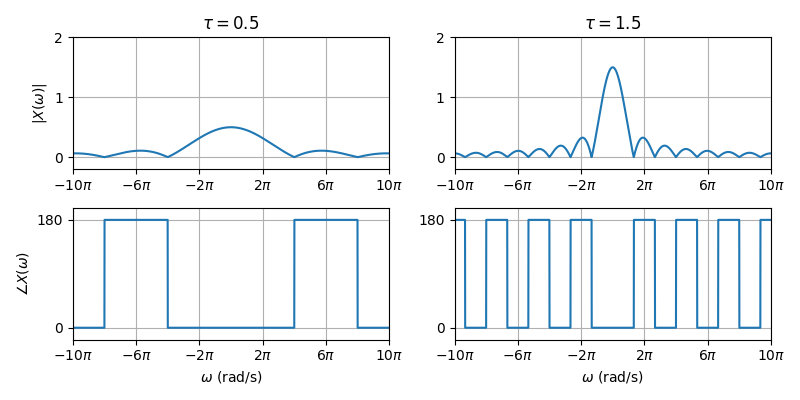
\includegraphics[height=5cm]{4.2.7-1.png}
\end{figure}

注意:
\begin{itemize}
    \item 所有图像的横坐标是角频$\omega $,单位是$\mathrm{rad}\cdot \mathrm{s}^{-1}$,为方便用弧度表示;
    \item $\underset{\tau \rightarrow 0}\lim p_{\tau}\left( t \right) =1,\underset{\tau \rightarrow 0}\lim X\left( \omega \right) =\delta \left( \omega \right) $。
\end{itemize}



\newpage
\section{Python应用——傅里叶变换函数}

本章的一个重点是能够将一个时域图形变换成傅里叶频谱并分析。
本节编写Python傅里叶变换函数,并借助Python快捷地获得傅里叶变换。

本节要点:
\begin{itemize}
    \item 学会Python编写傅里叶变换函数;
    \item 掌握分析方法。
\end{itemize}

%============================================================
\subsection{Python傅里叶变换函数}

由于Python没有傅里叶变换的函数,Numpy和Scipy都只有FFT,所以编写一个傅里叶变换的函数。

根据傅里叶变换公式my\_fourier编写如下函数:
\[
X\left( \omega \right) =\int_{-\infty}^{+\infty}{x\left( t \right) e^{-i\omega t}dt}
\]

\begin{python}
def my_fourier(
        x:np.ndarray, t:np.ndarray,
        w_range:tuple=(-5*np.pi, 5*np.pi), num:int=500
        ) -> tuple:

    w = np.linspace(w_range[0], w_range[1], num+1)
    F = np.zeros_like(w, dtype=np.complex64)
    dt = t[1] - t[0]

    for n in range(F.size):
        F[n] = np.dot(x, np.exp(0-w[n]*t*1.0j)) * dt
        pass

    return (F, w)
\end{python}

参数:
\begin{itemize}
    \item x:np.ndarray类型,表示信号$x\left( t \right) $的值;
    \item t:np.ndarray类型,表示信号$x\left( t \right) $的时间;
    \item w\_range:元组类型,表示$\omega $的取值范围,需要原点对称;
    \item num:整数类型,表示$\omega $的离散个数,也即$\omega $的采样个数。
\end{itemize}

函数流程:
\begin{enumerate}
    \item 首先根据w\_range和num生成w,我们做的傅里叶变换就在这个范围内,也即$\omega $的采样点,0点对称;
    \item 初始化傅里叶离散点,注意F的类型是np.complex64;
    \item 循环,核心是做积分;
    \item 返回(F,w)表示$F\left( \omega \right) ,\omega $。
\end{enumerate}

%============================================================
\subsection{分析方法}

通常有一类问题是已知一个连续信号的时域波形图,要分析它的频域。借助我们的函数,一般步骤如下:
\begin{enumerate}
    \item 根据图形写出连续信号的时域函数;
    \item 用my\_fourier()求傅里叶变换;
    \item 用Matplotlib画出幅频图和相频图分析。
\end{enumerate}

%============================================================
\subsection{例}

\begin{example}
假设有信号$x\left( t \right) =p_2\left( t \right) $,用Python计算傅里叶变换,并作图。
\end{example}

用Python求解傅里叶变换并作图:

\begin{python}
t    = np.arange(-20, 20, 0.01)
x    = np.where(t<-1, 0, np.where(t>1, 0, 1))
X, w = my_fourier(x, t, w_range=(-6*np.pi, 6*np.pi), num=1000)

axs[0].plot(t, x)
plot_mag_phs(w, np.abs(X), np.angle(X, deg=True), ...)
\end{python}

\begin{figure}[h]
\centering
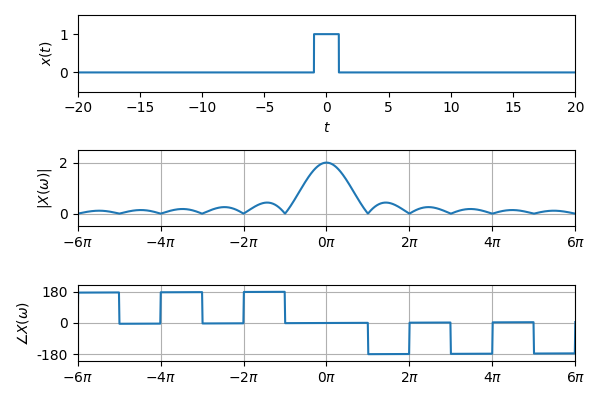
\includegraphics[height=5cm]{4.3.3-1.png}
\end{figure}

~

\begin{example}
设函数有如下图形,用Python分析傅里叶变换。
\begin{figure}[h]
\centering
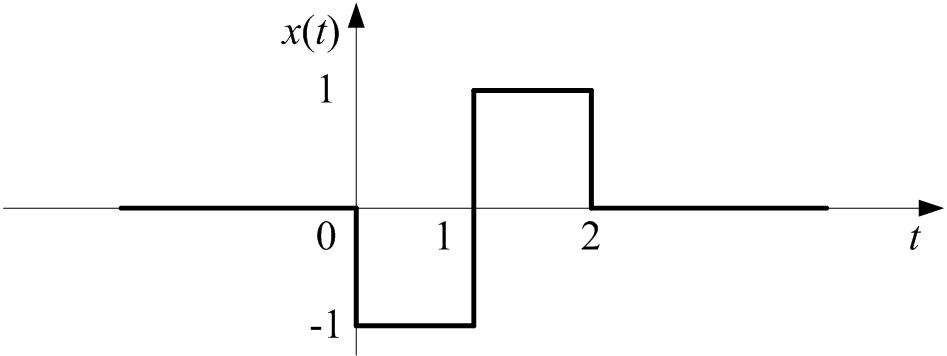
\includegraphics[height=2.5cm]{4.3.3-2.png}
\end{figure}
\end{example}

根据图形得到时域函数$x\left( t \right) =-u\left( t \right) +2u\left( t-1 \right) -u\left( t-2 \right) $,用Python求解傅里叶变换并作图:

\begin{python}
t    = np.arange(-20, 20, 0.01)
x    = np.where(t<0, 0, np.where(t<1, -1, np.where(t<2, 1, 0)))
X, w = my_fourier(x, t, w_range=(-6*np.pi, 6*np.pi))

axs[0].plot(t, x)
plot_mag_phs(w, np.abs(X), np.angle(X, deg=True), ...)
\end{python}

\begin{figure}[h]
\centering
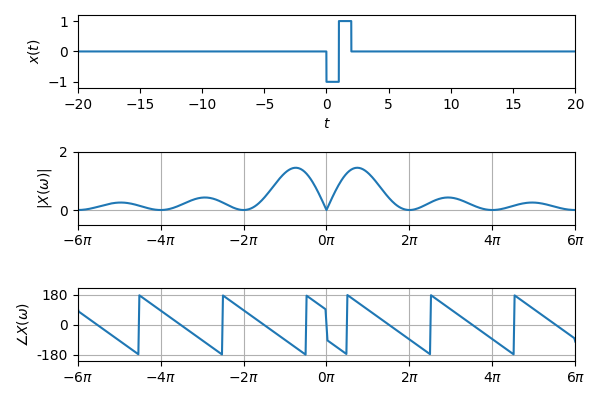
\includegraphics[height=5cm]{4.3.3-3.png}
\end{figure}

~

\begin{example}
设函数有如下图形,用Python分析傅里叶变换。
\begin{figure}[h]
\centering
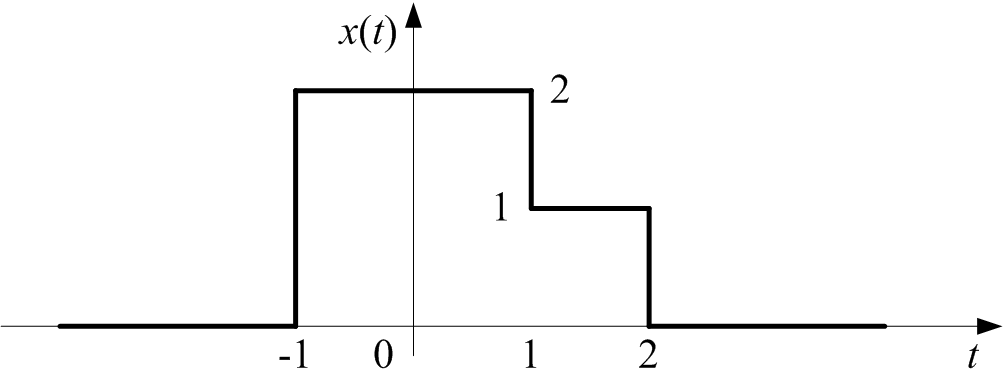
\includegraphics[height=2.5cm]{4.3.3-4.png}
\end{figure}
\end{example}

\begin{figure}[h]
\centering
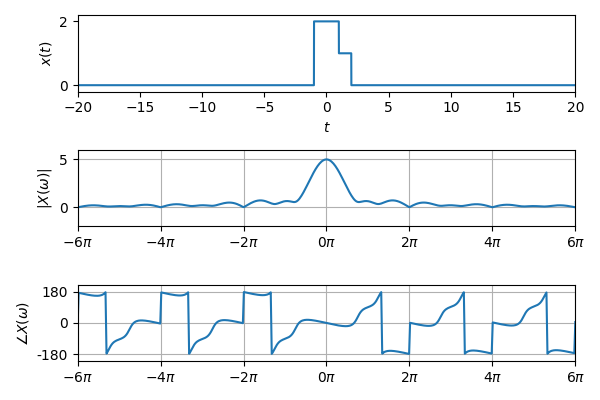
\includegraphics[height=5cm]{4.3.3-5.png}
\end{figure}

根据图形得到时域函数$x\left( t \right) =2u\left( t+1 \right) -u\left( t-1 \right) -u\left( t-2 \right) $,用Python求解傅里叶变换并作图:

\begin{python}
t    = np.arange(-20, 20, 0.01)
x    = np.where(t<-1, 0, np.where(t<1, 2, np.where(t<2, 1, 0)))
X, w = my_fourier(x, t, w_range=(-6*np.pi, 6*np.pi))

axs[0].plot(t, x)
plot_mag_phs(w, np.abs(X), np.angle(X, deg=True), ...)
\end{python}






\newpage
\section{本章小结}

傅里叶是频域分析的基础,必须深刻理解其含义,并熟练掌握计算方法。
时刻记住,数学本质上,傅里叶变换是函数的空间变换,将原本$x$空间的函数映射到三角函数(或指数函数)空间。
在信号与系统角度,具象化为时域到频域的变换,将原本对时间$t$的函数变换成对频率$\omega $的函数:
\[
\begin{array}{l}
	x=x\left( t \right)\\
	t\in \mathbb{R}\\
	x\in \mathbb{R}\\
\end{array} \quad \rightarrow \quad \begin{array}{l}
	X=X\left( \omega \right)\\
	\omega \in \mathbb{R}\\
	X\in \mathbb{C}\\
\end{array}
\]
一般来讲,$X\left( \omega \right) $的值域是复数,大小表示频率的振幅,角度表示频率的相位。

最后,需要特别注意$X\left( \omega \right) $的量纲$\mathrm{D}_x\cdot \mathrm{Hz}^{-1}$,及其物理意义“单位频率的信号,或者说信号的频率密度”。









